\title{Self Organizing Systems Exercise 1}
\author{
        Alexander Dobler 01631858\\
        Thomas Kaufmann 01129115 
}
\date{\today}

\documentclass[12pt]{article}

\usepackage{hyperref}
\usepackage{booktabs}
\usepackage{graphics}
\usepackage{multirow}
\usepackage{graphicx}
\usepackage{subcaption}
\usepackage{mwe}

\begin{document}
\maketitle

\section{Introduction \& Problem Description}
For exercise 1 of self-organizing systems we chose the task \textit{Sequence alignment for Genetic Data (DNA Lattice) Anonymization} in which we should solve the DNA lattice anonymization described in \cite{mainpaper} with two metaheuristic techniques from the lecture.
The task is to find a pairing of DNA sequences, such that the sum of distances between two DNA sequences of a pair over all pairs is as small as possible.

More specifically we are given a set of $n$ sequences described by strings which can have different length.
In a first step we have to align these sequences, such that all sequences have the same length.
This is done by introducing \textit{gap}-characters to increase the length of sequences.
In general this process is called multiple sequence alignment (MSA) and we do not describe how this is done here, but rather use a library as a black-box tool for this step.
Now, that every sequence has the same length, we can compute the distance between two sequences as described in \cite{mainpaper}.
The last and main step is to combine this set of sequences into pairs, such that the sum of distances of two sequences of a pair summed up over all pairs is minimal.
Obviously this is just an application of minimal weighted matching in a complete graph, where a graph is represented by $G=(V,E)$ as follows.
The set $V$ of nodes are described by the sequences and the set $E$ of edges is $V\times V$.
For an edge $e=\{u,v\}$ its weight $w(e)$ is just the distance between the sequences $u$ and $v$. 
We denote by $M \subset E$ a complete matching on a graph $G$, s.t. $2 \times |M| = |V|$, and by $c(M)$ the corresponding weight of the matching.

In the next sections we describe our solution approaches and main results.

\section{Test Data \& Preprocessing}
\label{sec:test-data}
As base set of data we chose DNA sequences from \url{https://www.kaggle.com/neelvasani/humandnadata} which consists of over 4000 human DNA sequences.
In a next step we created multiple instances of different size by selecting 10-300 random samples of these sequences.
Test-case sizes are always even, such that we do not have to bother about the leftover single sequence.
For each of these instances we performed some preprocessing with the python module \textit{Bio.SeqIO} from the package \textit{Bio} (\url{https://biopython.org/wiki/SeqIO}) and as suggested in ~\cite{mainpaper} compute multiple sequence alignments with the MSA-toolkit \emph{ClustalW}~\cite{clustalw}. 
In the last step we compute the cost-matrix between pairs of sequences as described in \cite{mainpaper}.
All of the algorithms described in the next section only use the cost-matrix to compute a pairing.
Although we chose instances of sizes comparable to the work of Bradley~\cite{mainpaper}, as shown below, instances turned out being relatively easy to solve where even the relatively simple construction heuristic obtains high quality solutions in little to no execution time. We then further investigated this behavior in more depth and found that a specially structured cost matrix due to the tree-based alignment procedure in \emph{ClustalW} often leads to edge-costs of $0$ between specific pairs in the graph, inherently favouring the nature of the DNALA construction heuristic. 

These test-cases can be found in the project under the folder \textit{data}:
Sequence alignments for each test-case are stored in the files \textit{human\_data\_XX.fasta} where \textit{XX} denotes the size of the test-case.
Similarly \textit{human\_data\_XX.cm} stores the cost-matrices in \textit{pickle}-format (\url{https://docs.python.org/3/library/pickle.html}).

\section{DNALA \& Exact Method}
We provide two preliminary methods to solve this problem which are used to benchmark the metaheuristik techniques:
\begin{itemize}
    \item An implementation of the DNALA algorithm as described in \cite{mainpaper} can be found in the \textit{algorithms} directory.
    We did implement the described randomness, but do not use multiple runs of the algorithm, but instead only run the algorithm for a testset once to determine its capability.

    \item As DNALA is only a heuristic and is not guaranteed to find an optimal solution we furthermore use a maximum weighted matching implementation provided by the package \textit{networkx} (\url{https://networkx.org/documentation/stable//index.html}) to compute an exact solution used for optimality gaps in benchmarking.
\end{itemize}

\section{Genetic Algorithm}
The first metaheuristic technique with which we solve the problem is a genetic algorithm.
For this we use the \textit{deap}-package for python (\url{https://deap.readthedocs.io/en/master/}) which provides a framework for creating genetic algorithms.
The well-know genetic algorithm compononents are implemented as follows:
\begin{itemize}
    \item \textbf{Solution representation}: A solution consists of $\frac{n}{2}$ pairs such that each node (sequence) appears in exactly one pair.
    \item \textbf{Fitness}: The fitness is just the sum of distances between pairs of points. 
    This in fact also represents the value of the corresponding weighted matching.
    \item \textbf{Crossover}: Given a pair of individuals $M_i$ and $M_j$, we derive a successor individual $M_{i'}$ with the following procedure:
    \begin{enumerate}
    	\item Select a subset $M'_i \subset M_i$ of matchings from individual $M_i$, where each edge $e \in M_i$ is selected with a probability of $0.5$. 
    	\item We then try to identify matchings $e \in M_j$ composed of edges not contained in $M'_i$, which are entirely preserved for the offspring $M_{i'}$.
    	\item Finally, we identify the remaining unmatched vertices and pair them randomly. 
    \end{enumerate}
    It is worth to notice that different variations of this approach were tested, considering orders of matchings in the solution representation as well as alternative strategies to pair remaining vertices, but no significant improved was obtained. 
    \item \textbf{Mutation}: Given an individual $M$, selects a random pair $e=\{u,v\}$, $e'=\{u',v'\} \in M$ of matchings based on a given mutation probability and constructs an offspring $M'$ by performing 1) an arbitrary or 2) the best two-opt in the subgraph induced by vertices $V=\{u,v,u',v'\}$. Experiments showed slight advantages for the intensifying mutation approach (i.e. the best two-opt neighbour) at only a negligible increase in computational cost. 
\end{itemize}
Furthermore we used a tournament selection strategy with tournament size of $k=3$ and have the option to select different population sizes and mutation rates for running the algorithm.

\section{Ant Colony Optimization}
At first we did not know how to solve the problem with ant colony optimization.
But then we realized that a weighted matching in a complete graph is just a tour visiting every vertice, where every second edge will have weight 0.
This was really convenient, as ant colony optimization is well-known to perform well on the TSP-problem.
Furthermore there are a lot of implementations available, which provide ACO-methods to solve the TSP-problem.
For our purposes it was enough to alter the implementation provided by the \textit{pants}-package (\url{https://pypi.org/project/ACO-Pants/}) in a way, such that we could solve the minimum weighted matching problem.

Our alteration can be described as follows.
When solving the TSP-problem every ant starts at a specific node and tries to find a best tour.
This means that at a specific point of the algorithm each ant has currently visited an acyclic path.
Now this path has either even or odd length.
This means when an ant can chose its next edge there are two different strategies:
\begin{itemize}
    \item If the path until now has even length, then choose the usual strategy to select the next node to visit (pheromones in ACO with $\alpha$- and $\beta$-values).
    \item If the path until now has odd length, then go to any not yet visited node.
    This resembles the fact that every other edge of the tour will have weight 0.
\end{itemize}
Of course we also have to alter the cost of a tour, in particular that every other edge has weight 0, to guide the algorithm to an optimal solution.

One might think that this construction of an algorithm to solve the minimum weighted matching problem is pretty superficial, but we will see that its performance is not too bad.

\section{Local Search}
While population based metaheuristics are usually great to identify high quality solution components in widely distributed solution spaces, they tend to end up in suboptimal regions, where simple intensification procedures like local search heuristics can significantly improve the solution quality. To this end, it is so common that population based metaheuristics are combined with local search procedures that for genetic algorithms the term \emph{memetic algorithm} has been established in the literature. In this work, we used a relatively simple two-opt neighbourhood structure with a constant time neighbour evaluation scheme and a first-improvement step function to improve populations of both the ACO as well as the GA. 

\section{Results \& Conclusion}
To evaluate the described approaches, experiments with a set of $12$ differently sized instances were run for different kinds of algorithm configurations. 
We used the optimality gap as a scale invariant performance measure describing the relative distance to the global optimum. 
As for particularly large instances, some configurations did converge towards the global optimum.
All experiments were run with a wallclock time of $300 s$ and $5$ repetitions each for statistical stability. Execution times do not include preparation time of cost matrices, since they have been precomputed and stored for reuse. All experiments were run on a Windows 10 machine with AMD Ryzen 3700X CPU in single-threaded mode. 

\subsection{Comparison of GA, ACO and DNALA}

Table~\ref{tab:main} compares both the GA as well as the ACO to the DNALA baseline, where we show the median values, for the optimality gap, the execution time as well as the iteration where the best solution was obtained. 

Main observations:
\begin{itemize}
	\item Purely population-based metaheuristic approaches work quite well for moderate sized instances, but solution quality declines significantly with increasing instance sizes. While for smaller instances, some instances could even be solved to optimality, for large instances the gap increases even above $100\%$ optimality gap. 
	\item Both approaches show the same behaviour with respect to the overall number of iterations conducted in the given period, where in smaller instances optimal solutions are obtained relatively fast and as the instance size increases, also the number of iterations until premature termination due to optimality increases. At some point, however, instances become more difficult and more expensive in terms of computational cost, such that the iteration count then steadily decreases, which in turn also affects solution quality. 
	\item It can be observed that our GA does not suffer from premature convergence as the iteration where the best solution was obtained tends to be close to the overall iteration count. This suggests that more iterations could still improve the solution quality. 
	\item Local search generally improves quality significantly, allowing to solve even larger instances almost to optimality. However, iteration count drops to a level suggesting our GA being basically just a \emph{fancy} random restart procedure. 
	\item The effectiveness of two-opt local search	backs up our observation of the biased instance generation procedure with \textit{ClustalW} mentioned in Section~\ref{sec:test-data}, since this simple neighborhood is able to identify the respective pairs of minimal cost easily. Furthermore, DNALA + LS seems to be quite good combtination 
\end{itemize}

\begin{table}
\centering
\resizebox{\columnwidth}{!}{%
\begin{tabular}{llr|rrrrr|rrrrr}
\toprule
   &     &          & \multicolumn{5}{|c|}{Without Local Search} & \multicolumn{5}{|c}{With Local Search} \\
   &     &  Optimum &  Fitness &    Gap &   Time &  $I_{opt}$ &  $I_{total}$ &  Fitness &   Gap &   Time &  $I_{opt}$ &  $I_{total}$ \\
ALG & n &          &          &        &        &            &          &       &        &            \\
\midrule
GA & 10  &     1994 &     1994 &   0.00 &   0.00 &          1 &                  1 &     1994 &  0.00 &   0.00 &          0 &                  0 \\
   & 20  &    11758 &    11758 &   0.00 &   0.00 &         13 &                 13 &    11758 &  0.00 &   0.00 &          0 &                  0 \\
   & 30  &    19032 &    19032 &   0.00 &   2.00 &         33 &                 33 &    19032 &  0.00 &   1.00 &          0 &                  0 \\
   & 40  &    20892 &    20892 &   0.00 &   5.00 &         54 &                 54 &    20892 &  0.00 &   3.00 &          0 &                  0 \\
   & 50  &    34198 &    34198 &   0.00 &  18.00 &        124 &                124 &    34198 &  0.00 &   3.00 &          0 &                  0 \\
   & 60  &    42382 &    44060 &   3.96 & 300.00 &        141 &               1795 &    42382 &  0.00 &  10.00 &          1 &                  1 \\
   & 70  &    47234 &    47498 &   0.56 & 300.00 &        221 &               1744 &    47234 &  0.00 &  15.00 &          1 &                  1 \\
   & 80  &    53538 &    53538 &   0.00 &  62.00 &        291 &                347 &    53538 &  0.00 &  23.00 &          2 &                  2 \\
   & 90  &    69731 &    70489 &   1.09 & 300.00 &        477 &               1322 &    69731 &  0.00 &  36.00 &          2 &                  2 \\
   & 100 &    83495 &    90825 &   8.78 & 300.00 &        314 &                314 &    83495 &  0.00 &  56.00 &          3 &                  3 \\
   & 150 &   104772 &   164686 &  57.19 & 300.00 &        141 &                141 &   104772 &  0.00 & 183.00 &          6 &                  6 \\
   & 200 &   130178 &   285042 & 118.96 & 300.00 &        142 &                142 &   133848 &  2.82 & 300.00 &          7 &                  7 \\
   \midrule
ACO & 10  &     1994 &     1994 &   0.00 &   0.00 &          0 &                  0 &     1994 &  0.00 &   0.00 &          0 &                  0 \\
   & 20  &    11758 &    11758 &   0.00 &   0.00 &          0 &                  0 &    11758 &  0.00 &   0.00 &          0 &                  0 \\
   & 30  &    19032 &    19032 &   0.00 &   0.00 &          1 &                  1 &    19032 &  0.00 &   0.00 &          0 &                  0 \\
   & 40  &    20892 &    20892 &   0.00 &   8.00 &         89 &                 89 &    20892 &  0.00 &   0.00 &          0 &                  0 \\
   & 50  &    34198 &    34280 &   0.24 & 300.00 &       1380 &               1856 &    34198 &  0.00 &   1.00 &          0 &                  0 \\
   & 60  &    42382 &    45370 &   7.05 & 300.00 &        326 &               1358 &    42382 &  0.00 &   1.00 &          0 &                  0 \\
   & 70  &    47234 &    50798 &   7.55 & 300.00 &        361 &               1271 &    47234 &  0.00 &   2.00 &          0 &                  0 \\
   & 80  &    53538 &    60098 &  12.25 & 300.00 &        684 &                775 &    53538 &  0.00 &   3.00 &          0 &                  0 \\
   & 90  &    69731 &    83165 &  19.27 & 300.00 &        500 &                598 &    69731 &  0.00 &   5.00 &          0 &                  0 \\
   & 100 &    83495 &   107569 &  28.83 & 300.00 &        428 &                512 &    83495 &  0.00 &  22.00 &          4 &                  4 \\
   & 150 &   104772 &   157702 &  50.52 & 300.00 &         57 &                194 &   108990 &  4.03 & 300.00 &         18 &                 32 \\
   & 200 &   130178 &   218002 &  67.46 & 300.00 &         49 &                125 &   171176 & 31.49 & 300.00 &         20 &                 24 \\
   \midrule
DNALA & 10  &     1994 &     1994 &   0.00 &   0.00 &          - &                  - &     1994 &  0.00 &   0.00 &          - &                  - \\
   & 20  &    11758 &    11758 &   0.00 &   0.00 &          - &                  - &    11758 &  0.00 &   0.00 &          - &                  - \\
   & 30  &    19032 &    19032 &   0.00 &   0.00 &          - &                  - &    19032 &  0.00 &   0.00 &          - &                  - \\
   & 40  &    20892 &    22066 &   5.62 &   0.00 &          - &                  - &    21164 &  1.30 &   0.00 &          - &                  - \\
   & 50  &    34198 &    35336 &   3.33 &   0.00 &          - &                  - &    34198 &  0.00 &   0.00 &          - &                  - \\
   & 60  &    42382 &    44666 &   5.39 &   0.00 &          - &                  - &    42890 &  1.20 &   0.00 &          - &                  - \\
   & 70  &    47234 &    47252 &   0.04 &   0.00 &          - &                  - &    47244 &  0.02 &   0.00 &          - &                  - \\
   & 80  &    53538 &    55448 &   3.57 &   0.00 &          - &                  - &    53538 &  0.00 &   0.00 &          - &                  - \\
   & 90  &    69731 &    71779 &   2.94 &   0.00 &          - &                  - &    69747 &  0.02 &   0.00 &          - &                  - \\
   & 100 &    83495 &    86513 &   3.61 &   0.00 &          - &                  - &    85293 &  2.15 &   0.00 &          - &                  - \\
   & 150 &   104772 &   105824 &   1.00 &   0.00 &          - &                  - &   104940 &  0.16 &   0.00 &          - &                  - \\
   & 200 &   130178 &   134640 &   3.43 &   0.00 &          - &                  - &   130194 &  0.01 &   0.00 &          - &                  - \\

\bottomrule
\end{tabular}%
}
\caption{Comparison of GA and ACO against the DNALA baseline in $12$ different instances.}\label{tab:main}
\end{table}


\subsection{Comparison of GA Mutation Operators}
The previous section showed that our GA is not subject to premature convergence. However, the effectiveness of the two-opt neighbourhood structure and the fact that improvements occur frequently in the last iterations, we suspected that our GA was actually a multi-solution, random-neighbour local search. To this end, we compared the random two-opt move mutation operator against the best two-opt move one. Table~\ref{tab:mutation-operator} compares median values for fitness, optimality gap, execution time and iteration characteristics for both types for moderate and large instance types. 

Main observations:
\begin{itemize}
	\item The randomized approach general performs quite similarly, however, tends to require more iterations for comparable solution qualities (e.g. $n=70$)
	\item For smaller instances, the locally-improving moves seem to be slightly advantageous in terms of convergence pace. 
	\item As the instance size increases, the effect of small locally-improving moves seem to vanish and both quality as well as iteration characteristics seem to align. 
\end{itemize}

\begin{table}
\centering
\resizebox{\columnwidth}{!}{%
\begin{tabular}{llr|rrrrr}
\toprule
      &     &   Optimum &   Fitness &    Gap &   Time &   $I_{opt}$ &  $I_{total}$  \\
type & n &           &           &        &        &            &                    \\
\midrule
Random & 70  &  47234.00 &  47371.00 &   0.29 & 300.00 &     278.50 &            2203.50 \\
      & 80  &  53538.00 &  55116.00 &   2.95 & 300.00 &     564.00 &            1650.00 \\
      & 90  &  69731.00 &  70490.00 &   1.09 & 300.00 &     599.00 &            1012.00 \\
      & 100 &  83495.00 &  94405.00 &  13.07 & 300.00 &     501.00 &             629.50 \\
      & 150 & 104772.00 & 180576.00 &  72.35 & 300.00 &     149.00 &             149.00 \\
      & 200 & 130178.00 & 280278.00 & 115.30 & 300.00 &     142.50 &             142.50 \\
         \midrule
Best  & 70  &  47234.00 &  47366.00 &   0.28 & 221.00 &     320.00 &            1523.50 \\
      & 80  &  53538.00 &  53538.00 &   0.00 &  88.00 &     295.50 &             364.50 \\
      & 90  &  69731.00 &  71061.00 &   1.91 & 300.00 &     486.00 &            1492.50 \\
      & 100 &  83495.00 &  89561.00 &   7.27 & 300.00 &     401.50 &            1002.50 \\
      & 150 & 104772.00 & 192572.00 &  83.80 & 300.00 &     135.50 &             135.50 \\
      & 200 & 130178.00 & 279480.00 & 114.69 & 300.00 &     143.50 &             143.50 \\
\bottomrule

\end{tabular}%
}
\caption{Comparison of the random and best two-opt move in the GA mutation operator.}\label{tab:mutation-operator}
\end{table}


\subsection{Population Size}
As the name might suggest, population size is obviously a crucial parameter in population-based metaheuristics. On the one hand, an increased population size allows vaster search diversity and allows to cover more areas in the solution space at once, obviously increasing likelihood to identifying new promising regions. 
On the other hand, metaheuristics usually require lots of iterations to continuously improve the solution quality, which obviously is a major limiting factor for large population sizes. 
In Figure~\ref{fig:population} we compare the impact of different population sizes on the optimality gap over time in single executions on two different instances (usually a time bucket average would be more appropriate for statistical stability, but we assumed this was beyond the scope if this exercise).

Main observations:
\begin{itemize}
	\item Too large population sizes inherently lead to increased computational costs, thus slowing down individual iterations, as can be observed in Figure~\ref{fig:population-b}
	\item The increased population sizes, however, increase search diversity, thus may improve solution quality (compare again Figure~\ref{fig:population-b}). Of course this depends on the structure of the solution space, e.g. big-valley vs. widely distrusted.
	\item Independent of the population size, it can be observed that the GA tends to perform small steps towards improving solutions until convergence towards an (local or global) optimum sets in, while the ACO seems to require large periods to obtain improving solutions. This could be either an indicator for a suboptimal model or some hyper-parameter issue. In a more elaborated study, we would use for instance the R-package irace for proper parameter tuning. 
\end{itemize}

  \begin{figure*}
        \centering
        \begin{subfigure}[b]{0.475\textwidth}
            \centering
            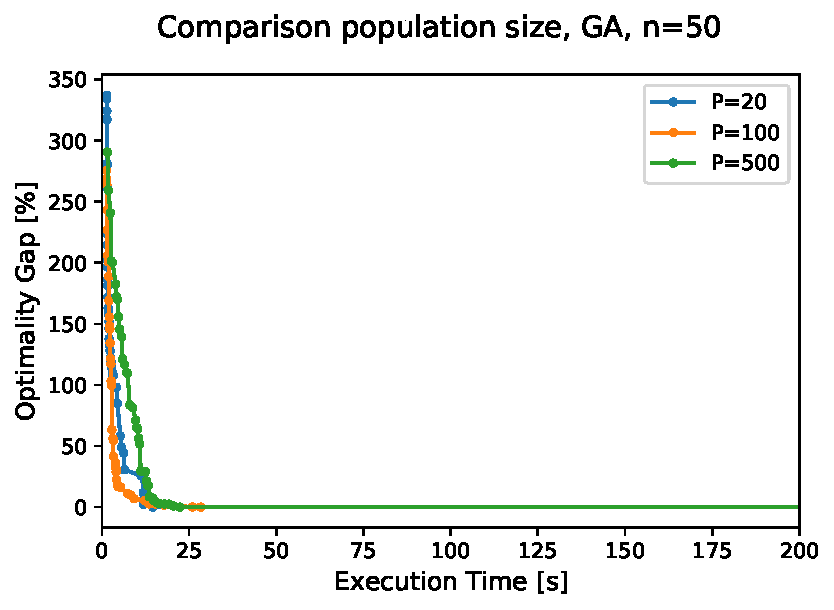
\includegraphics[width=\textwidth]{figures/ga_50_population_comparison.pdf}
            \caption%
            {{\small }}    
            \label{fig:population-a}
        \end{subfigure}
        \hfill
        \begin{subfigure}[b]{0.475\textwidth}  
            \centering 
            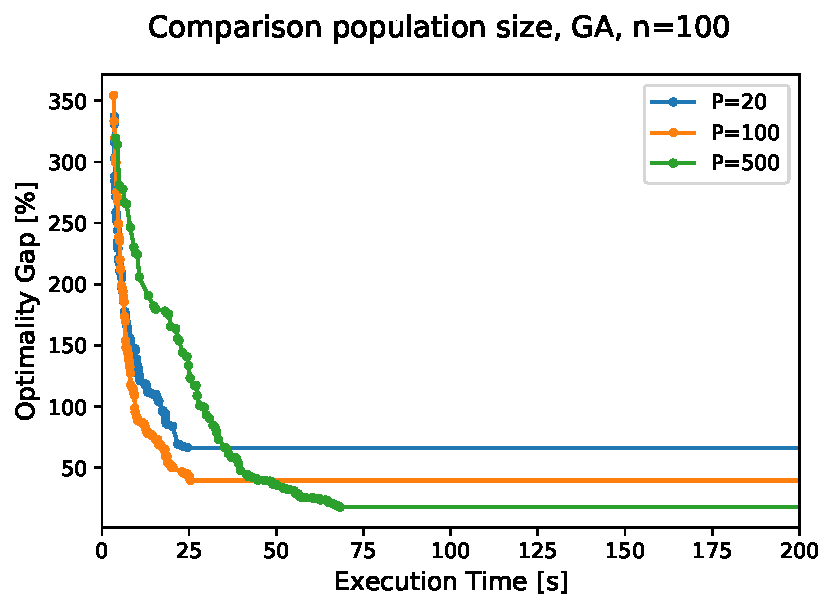
\includegraphics[width=\textwidth]{figures/ga_100_population_comparison.pdf}
            \caption%
            {{\small }}     
            \label{fig:population-b}
        \end{subfigure}
        \vskip\baselineskip
        \begin{subfigure}[b]{0.475\textwidth}   
            \centering 
            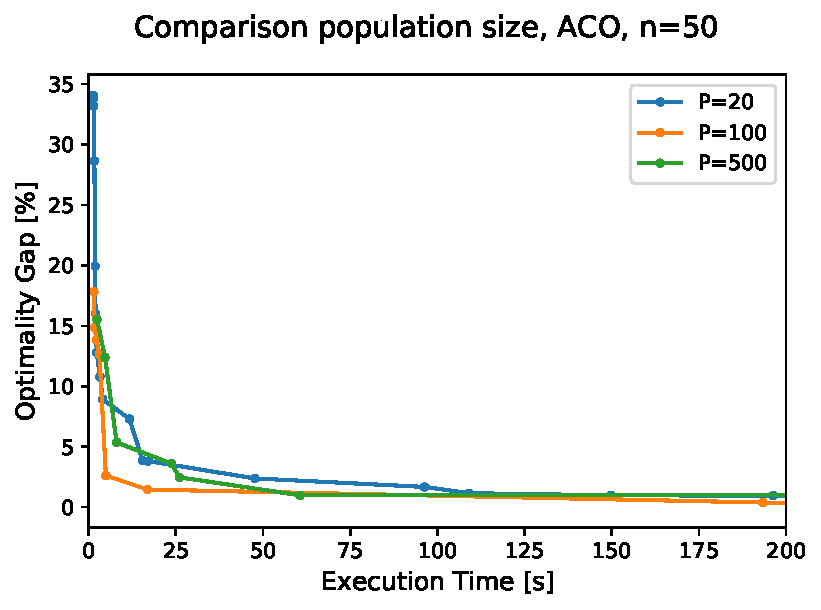
\includegraphics[width=\textwidth]{figures/aco_50_population_comparison.pdf}
            \caption%
            {{\small }}      
            \label{fig:population-c}
        \end{subfigure}
        \hfill
        \begin{subfigure}[b]{0.475\textwidth}   
            \centering 
            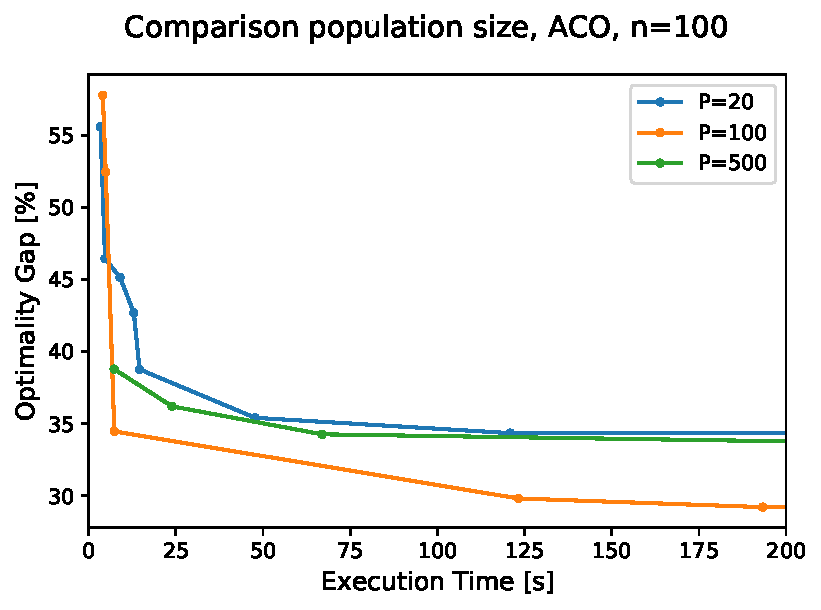
\includegraphics[width=\textwidth]{figures/aco_100_population_comparison.pdf}
            \caption%
            {{\small }}    
            \label{fig:population-d}
        \end{subfigure}
        \caption
        {\small Optimality gap over time for different population sizes on instances with $n=50$ and $n=100$ vertices. } 
        \label{fig:population}
    \end{figure*}


\subsection{Hyper-parameters}
In addition to some manual tweaking of hyper-parameters, we performed a very limited comparison of selected hyper-parameters of both the GA and the ACO. 
The default mutation rate corresponds to $2/|V|$, multiplied by a tunable parameter $r \in \{1,4,8\}$. The integer values for alpha and beta define the relative importance of pheromones and distances respectively. 

Main observations:
\begin{itemize}
	\item We can clearly see that with too high mutation rate ($r=8$) the genetic algorithm does not converge to the optimum, whereas for $r=1$ and $r=4$ the performance is similar.
	\item For ACO alpha=1 and beta=4 or beta=8 clearly outperforms all other parameter choices, suggesting the importance of distance information rather than pheromones again likely due to specially structured instances.
\end{itemize}

 \begin{figure*}
        \centering
        \begin{subfigure}[b]{0.475\textwidth}
            \centering
            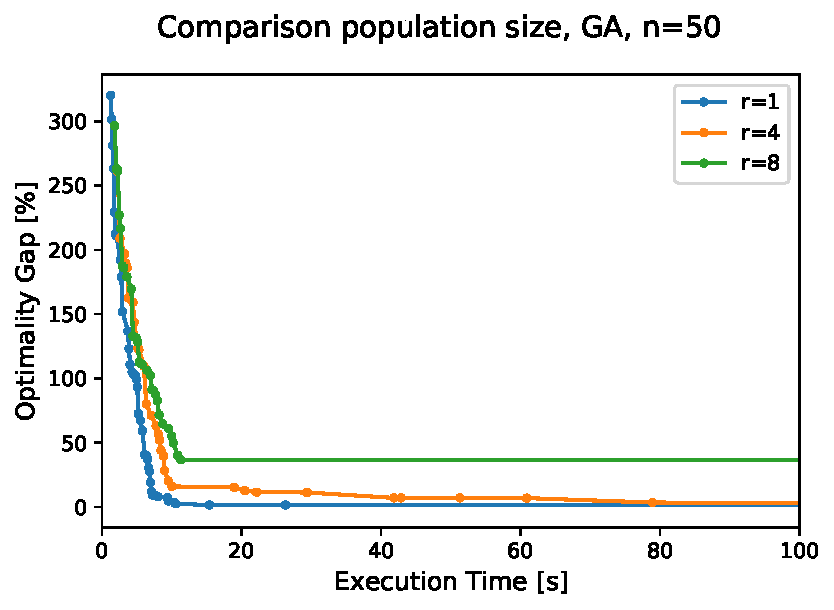
\includegraphics[width=\textwidth]{figures/ga_50_mutation_rate_comparison.pdf}
            \caption%
            {{\small }}    
            \label{fig:mean and std of net14}
        \end{subfigure}
        \hfill
        \begin{subfigure}[b]{0.475\textwidth}  
            \centering 
            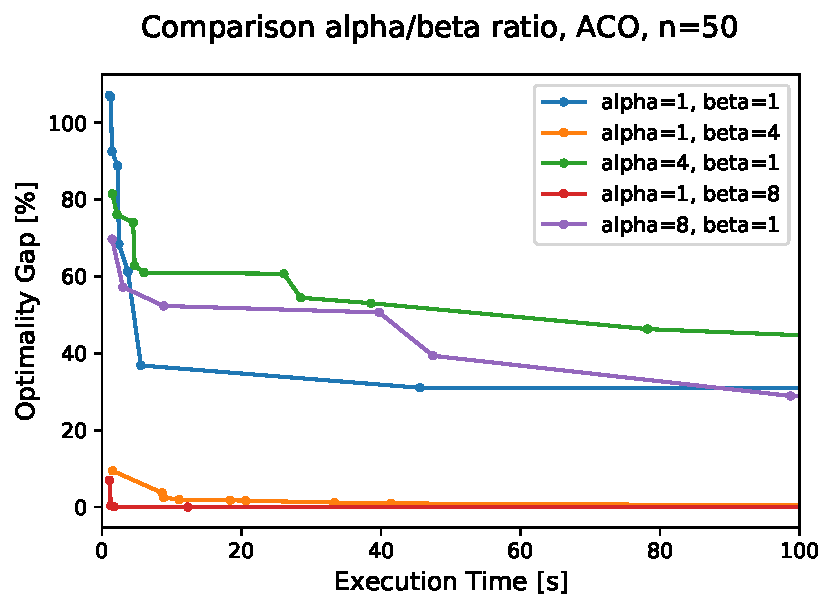
\includegraphics[width=\textwidth]{figures/aco_50_alpha_beta_ratio_comparison.pdf}
            \caption%
            {{\small }}     
            \label{fig:mean and std of net24}
        \end{subfigure}
        \caption
        {\small Optimality gap over time for different parameters with $n=50$ vertices. } 
        \label{fig:mean and std of nets}
    \end{figure*}

\section{Conclusion}
We have seen two metaheuristic techniques to solve the minimum weighted matching problem, namely ACO and genetic algorithms.
Both approaches performed similarly and converged to optimal solutions in appropriate times even for larger instances.

\bibliographystyle{abbrv}
\bibliography{main}


\end{document}
  